\chapter{Related Work}

\label{ch:relatedwork}

\section{Workload-Aware Frameworks}

\subsection{Database Cracking}

From Idreos et al, Cracking is a relational database auto-tuning technique which performs online restructuring of a relational table into disjoint pieces, storing information about each piece within a separate data-structure called the cracker index.

When a column is queried, it is copied into a version of the column called the cracker column. The cracker column is then scanned, restructuring it in-place to position the retrieved elements in contiguous memory. The indices of the bounds of the newly formed contiguous region are stored within the cracker index to optimise future queries by reducing the amount of the column needing to be scanned.

Figure \ref{fig:cracking_img} shows two queries being run against a column within a system employing database cracking. We can see that Q1 copies the original column into a cracker column, which is then partitioned into pieces from the scan, of which information is known about the contents. Q2 further breaks up the column into pieces, and again the information about the newly formed partitions is stored in the cracker index.

\begin{figure}[h]
  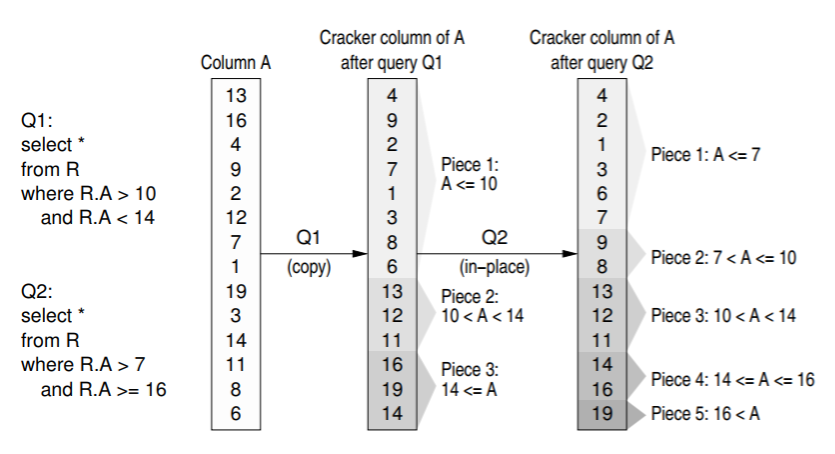
\includegraphics[width=\textwidth]{cracking_img}
  \caption{Example of a column being cracked}
  \label{fig:cracking_img}
\end{figure}

Database cracking is discussed in much more detail in Chapter \ref{ch:background}.

\subsection{Group-by-Query}

In-part inspired by cracking was the thesis work of Aluç, who proposed a group-by-query (G-by-Q) representation for RDF data, for which the structure of individual database records, as well as the way records are serialized on the storage system are dynamically determined based on the workload. 

Using G-by-Q, the way database records are serialised and their contents are determined dynamically by the workload. The format of database records is determined by the queries on the database. The diagram below shows an example of the storage for a database which has had two types of queries applied to it. $P_{1}$ to $P_{3}$ are the results of a linear query, whereas $P_{4}$ and $P_{5}$ are both the results of star-shaped queries.

\begin{figure}[h]
  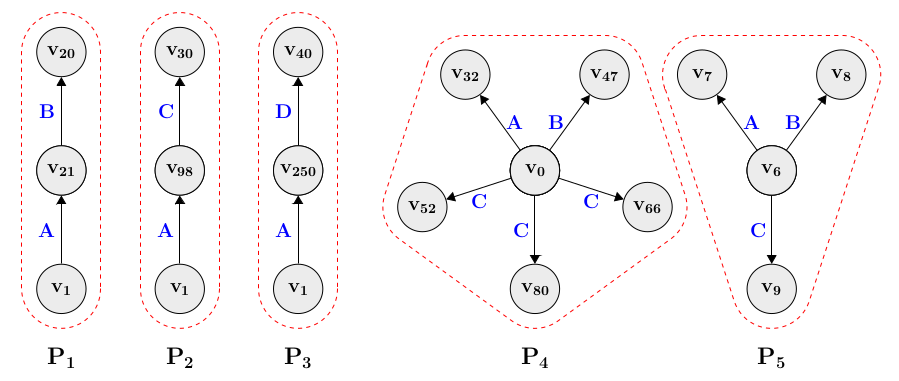
\includegraphics[width=\textwidth]{g_by_q_img}
  \caption{Example of G-by-Q storage representation}
  \label{fig:g_by_q_img}
\end{figure}

This technique proved to be fast and robust against other popular frameworks for querying RDF data, however, the system is complicated - Aluç's implementation was reported to be over 35,000 lines of C++. In this work we aimed to produce simpler contributions. Additionally, the G-by-Q technique is used for point-type queries, which seek to find all instances of certain subgraphs within a graph based on node labels, whereas our contributions are focused on traversal queries, which move through the graph by following edges and making computations based off the node and edge properties.

\section{Graph Processing}

\subsection{Ligra Framework}

Ligra is a lightweight graph processing framework for shared-memory multi-core machines for graph traversal algorithms, such as pagerank and BFS. Ligra takes the form of a simple API of three routines: size, edgeMap and vertexMap, as described in the paper.

\textbf{size}(U) returns the number of vertices in the set U.

\textbf{edgeMap}(G, U, F, C) applies the function F to all edges in G with source vertex in U and target vertex satisfying C.

\textbf{vertexMap}(U, F) applies the function F to every vertex in the set U.

A crucial advantage of the Ligra framework is that in the cases of both edgeMap and vertexMap, the supplied function can run in parallel, however, the user must ensure parallel correctness.

\subsection{Frequency Based Clustering}

Frequency based clustering constitutes physically reorganising the vertex data such that frequently accessed vertices are clustered together. In the case of traversal algorithms, as were studied specifically by this paper, the property by which to cluster vertices is their degree (in- or out-degree depending on the algorithm). By doing this clustering, cache contention between threads is reduced thanks to the improved locality between frequently accessed vertices. This improves cache utilisation and reduces the cycles spent stalled on memory. The authors found that real world graphs often exhibit inherent locality, and disturbing the structure of the vertex data too much causes performance to worsen. They determined that they achieved the best performance when they clustered together vertices at one end of the graph only if their degree exceeded the mean degree across all nodes.

\subsection{CSR segmenting}

This technique, by Kiriansky et al. just like frequency based clustering, aims to optimise the cache performance of a graph algorithm by making random accesses go only to the cache and by making all memory accesses sequential. It does this by working only on a single cache-sized segment of the vertex data at a time. By segmenting the graph into cache-sized subgraphs, all the required vertex data for the processing of a single subgraph can be stored in the cache.

This method requires preprocessing of the adjacency list, followed by the processing of each segment. Segments are processed one at a time, but the computation within the segment is fully parallelised. There is no cache-contention because the threads all share the same read-only working set (vertex data). We can avoid high merging cost after the computations by not using too many segments. The author's did experiments using a high number of segments which fit in the L2 cache, however, the best performance was achieved by using fewer segments, each of which fit in the LLC and contained a large number of edges. After the segments are all processed a low-cost cache-aware merge is used to combine the intermediate results from each segment.

\section{Graph Indices}

\subsection{Space filling curve layouts}

The most famous example of this is the Hilbert Curve, which is a continuous mapping between a number and a point on a 2D square. Numbers which are close by are mapped closely together - in this way the Hilbert ordering of an index of an adjacency list is somewhat locality preserving. We can use a Hilbert ordering in order to improve locality on edge accesses, which therefore leads to improved cache performance.
